\section{Анализ экспериментов}
\subsection{Цель и постановка экспериментов}

Эксперименты проверяют два ожидаемых эффекта адаптивного перекодировщика:
охлаждение данных должно уменьшать расход места, а рост температуры или
частичная недоступность должны ограничивать переход в схемы с дорогим чтением.
Поэтому измеряются не только итоговые доли схем, но и динамика переходов,
стоимость фоновой работы и задержки пользовательского чтения.

Для сравнения используются три режима:
\begin{itemize}
    \item только реплики --- данные после записи остаются в состоянии
    \(Hy(3,LRCC(d,0,0))\);
    \item только LRCC(24,1,2) --- данные сразу переводятся в широкую
    фиксированную схему \(Hy(0,LRCC(24,1,2))\); если последняя группа объекта
    неполная, она физически дополняется нулевыми блоками;
    \item перекодировщик --- обычная работа локальных и глобального
    планировщиков, где состояние каждой схемы может меняться во времени.
\end{itemize}

Такое сравнение соответствует требованию сопоставить результаты экспериментов с
существующими подходами: фиксированная репликация представляет традиционный
вариант с быстрым чтением и высоким расходом места, а фиксированный LRCC(24,1,2)
представляет подход на основе кодов стираний с меньшим расходом места и более
дорогим восстановлением при отказах. Предлагаемый перекодировщик сравнивается с
ними как адаптивная надстройка, выбирающая состояние схемы в зависимости от
температуры данных и текущего давления по ресурсам.

В качестве основных метрик используются:
\begin{itemize}
    \item суммарно занятое место на дисках блоками данных, избыточности или
    репликами --- метаданные и прочий шум не измеряются;
    \item распределение схем по точным сигнатурам \(Hy(r,LRCC(d,l,g))\);
    \item распределение пользовательских логических блоков по тем же
    сигнатурам схем;
    \item число операций чтения, отнесённых к одному запрошенному
    логическому блоку;
    \item задержка чтения, рассчитанная в модели «выдачи логического
    блока клиенту»: потоковая выдача из реплик против барьера сборки для LRCC.
\end{itemize}

В отличие от счётчиков дисковых чтений, задержка чтения оценивается как время,
когда запрошенный логический блок становится доступен клиенту.

\subsection{Холодные данные}

Первый сценарий моделирует запись большого объекта и последующее простаивание.
Это базовая проверка того, что при нулевой температуре данных оптимизация
должна стремиться к уменьшению занимаемого места.

\begin{figure}[!htbp]
\begin{center}
   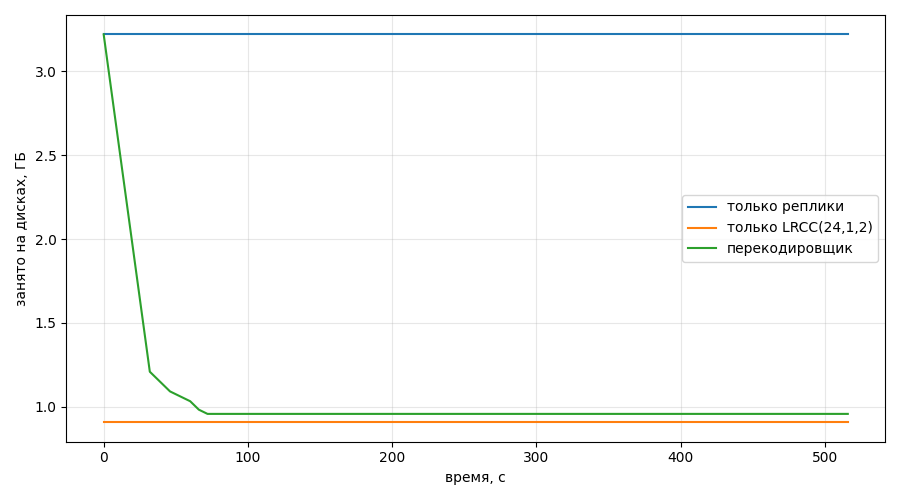
\includegraphics[width=0.92\textwidth]{images/experiments/cold_disk_used.png}
\caption{
\label{fig:cold-disk-used}
     Изменение занятого места после записи холодного объекта.}
\end{center}
\end{figure}

На рис.~\ref{fig:cold-disk-used} видно, что режим только с репликацией остаётся
на верхней границе по занимаемому месту, а режим только LRCC(24,1,2) задаёт
нижнюю границу. Перекодировщик начинает с того же состояния, что и репликация,
но затем постепенно переводит схемы в состояние с преобладанием проверочных
блоков и приближается к LRCC. Это показывает основную ожидаемую динамику: если
данные не читаются, реплики становятся избыточно дорогим способом хранения.
\FloatBarrier

\subsection{Длительная запись и фоновые переходы}

Следующий сценарий добавляет продолжительную запись новых объектов. Во время
записи перекодировщик не всегда успевает немедленно перевести все новые схемы в
LRCC, потому что фоновые переходы имеют задержку и ограничиваются числом
доступных локальных планировщиков.

\begin{figure}[!htbp]
\begin{center}
   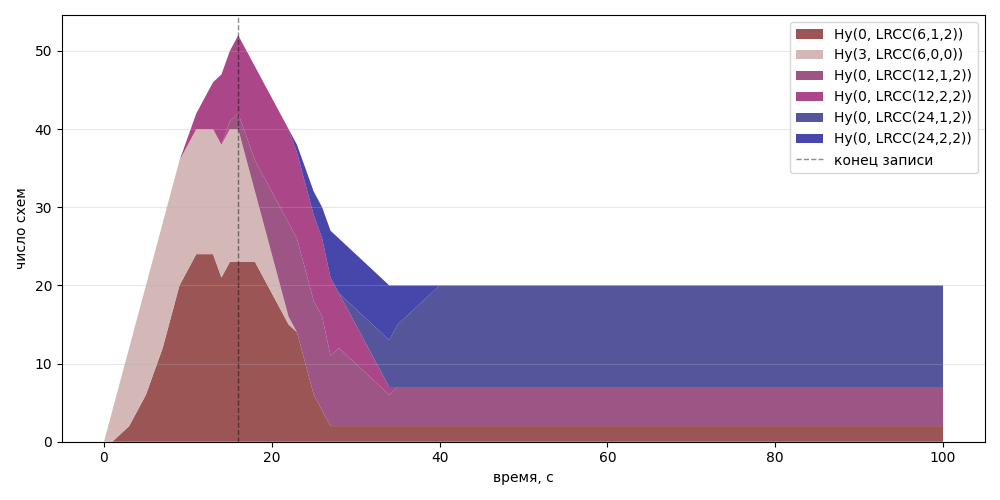
\includegraphics[width=0.92\textwidth]{images/experiments/continuous_scheme_distribution.png}
\caption{
\label{fig:continuous-scheme-distribution}
     Распределение точных сигнатур схем при продолжительной записи и
     последующем ожидании.}
\end{center}
\end{figure}

На рис.~\ref{fig:continuous-scheme-distribution} видно накопление схем с
преобладанием реплик во время активной записи. После окончания записи фоновые
переходы догоняют накопившуюся очередь, и почти все пользовательские блоки
переходят в широкие LRCC-состояния. Этот график полезен тем, что показывает не
только конечное состояние, но и инерционность системы: перекодирование является
фоновым процессом, а не мгновенной частью пути записи.
\FloatBarrier

\subsection{Неравномерная температура данных}

Равномерные случайные чтения часто размазывают температуру по объектам и не
создают ярко выраженных горячих или холодных областей. Поэтому отдельно
рассматривается нагрузка с распределением Ципфа
\cite{zipf1949human,breslau1999zipf}: логическое пространство объектов заранее
разбивается на куски, после чего вероятность чтения куска пропорциональна
обратной степени его ранга. Такой сценарий приближает модель к типичной
нагрузке систем хранения, где небольшая часть данных читается существенно чаще
остальных.

\begin{figure}[!htbp]
\begin{center}
   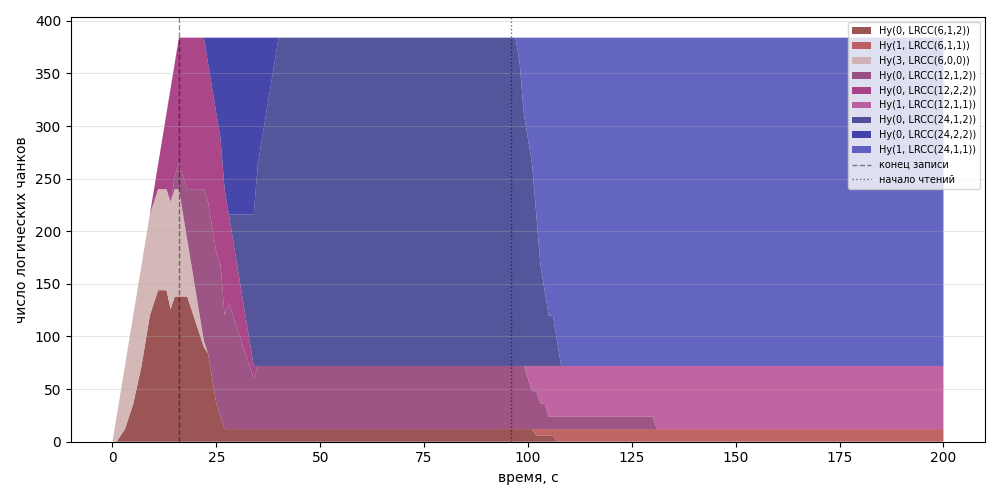
\includegraphics[width=0.92\textwidth]{images/experiments/logical_chunk_distribution.png}
\caption{
\label{fig:zipf-scheme-distribution}
     Распределение блоков данных по сигнатурам схем при чтениях по распределению Ципфа.}
\end{center}
\end{figure}

На рис.~\ref{fig:zipf-scheme-distribution} сначала при бездействии схемы
остывают, затем после начала чтения часть данных переходит в гибридные
состояния, так как для горячих областей выигрыш по чтению оказывается важнее
дополнительного расхода места. Это ключевой эксперимент для проверки
адаптивности: система реагирует не только на факт записи, но и на последующую
температуру отдельных схем.
\FloatBarrier

\subsection{Чтения при отказах}

Для оценки цены отказов моделируются сбои на случайных узлах: при
недоступности блока данных чтение восстанавливает его синхронно из локальных
или глобальных проверочных блоков, не меняя метаданные и не выполняя фоновое
восстановление. Отказ в экспериментах вносится как пометка узла недоступным.
В более интенсивном сценарии одновременно недоступны до трёх узлов с
LRCC-блоками данных, а набор отказавших узлов периодически меняется по кругу.

\begin{figure}[!htbp]
\begin{center}
   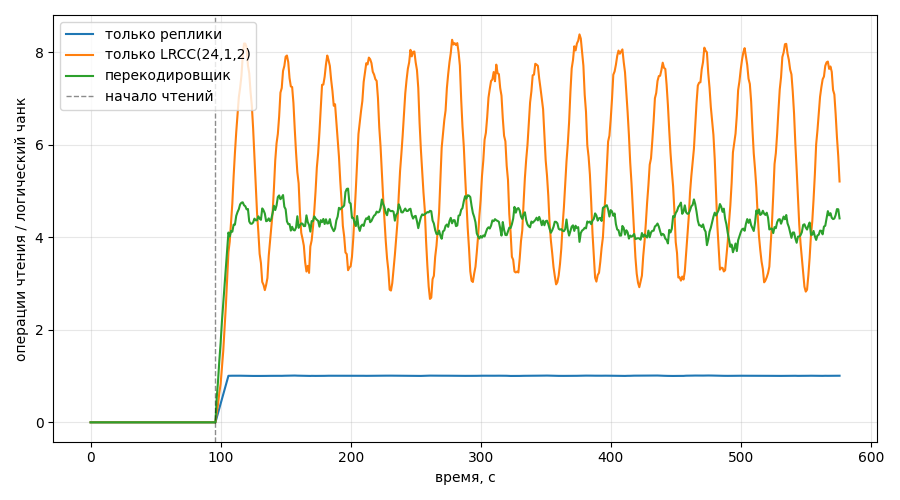
\includegraphics[width=0.92\textwidth]{images/experiments/avg_real_read_ops_smoothed.png}
\caption{
\label{fig:stress-read-ops}
     Сглаженное число операций чтения на логический блок при случайных чтениях
     и интенсивных отказах.}
\end{center}
\end{figure}

На рис.~\ref{fig:stress-read-ops} режим только LRCC(24,1,2) показывает пики,
потому что читает блоки данных и избыточности для восстановления. Схема
широкая, поэтому статистически очень вероятны отказы в схеме, располагающейся
почти по всем узлам. Репликация почти не чувствительна к такому сценарию, пока
среди доменов отказа, хранящих прямые размещения нужного блока, доступен хотя
бы один. Перекодировщик занимает промежуточное положение: часть данных хранится
компактно, но горячие или рискованные схемы могут оставаться в более удобном
для чтения состоянии.
\FloatBarrier

\subsection{Смешанный жизненный цикл}

Наиболее близкий к целевому поведению сценарий объединяет несколько фаз:
продолжительную запись, простой, чтения по распределению Ципфа и затем
равномерные случайные чтения. Он нужен, чтобы проверить, что система не
оптимизируется под один искусственный момент времени, а меняет состояние при
смене характера нагрузки.

\begin{figure}[!htbp]
\begin{center}
   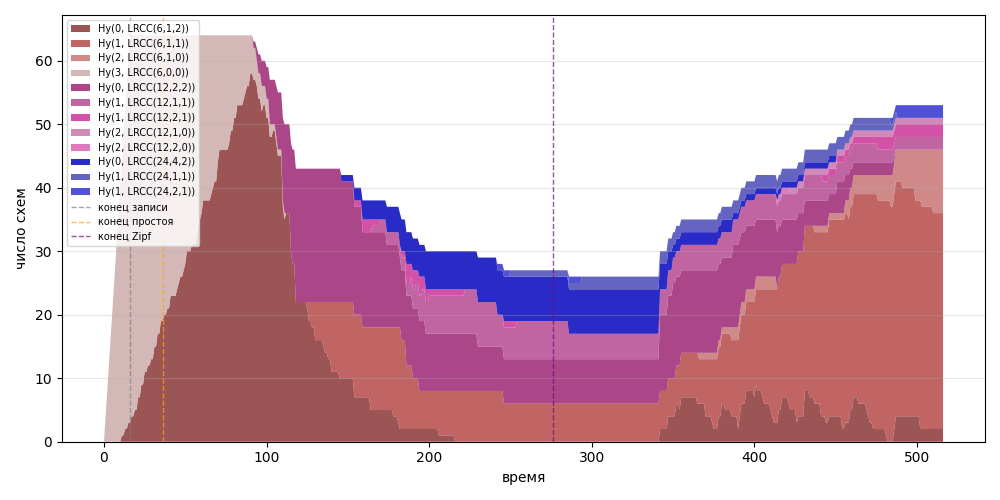
\includegraphics[width=0.92\textwidth]{images/experiments/scheme_distribution.png}
\caption{
\label{fig:mixed-scheme-distribution}
     Изменение распределения схем в смешанном сценарии:
     запись, простой, чтения по распределению Ципфа и случайные чтения.}
\end{center}
\end{figure}

На рис.~\ref{fig:mixed-scheme-distribution} после фазы записи и простоя схемы
уходят в широкие LRCC, что соответствует холодному хранению. Затем во время
чтений часть схем возвращается в гибридные состояния с преобладанием реплик
или разделяется на более узкие схемы. После смены распределения чтений меняется
и баланс типов схем. Более того, меняется и количество схем --- это связано с
их объединениями и разделениями. Этот график наиболее полно демонстрирует идею
конвертируемых кодов в данной работе
\cite{maturana2022convertible,kong2024lrcconvertible}: код не выбирается один
раз навсегда, а становится управляемым состоянием жизненного цикла данных.
\FloatBarrier

\subsection{Выводы по экспериментам}

Проведённые эксперименты подтверждают ожидаемое поведение предложенного
подхода. Во-первых, для холодных данных перекодировщик приближается к
эффективности LRCC по занимаемому месту. Во-вторых, при неравномерной
температуре он сохраняет часть схем в более дорогих по месту, но дешёвых по
чтению состояниях. В-третьих, при отказах чистый LRCC выигрывает по месту, но
платит ростом числа чтений при восстановлении и задержки; адаптивный режим
позволяет частично сгладить этот компромисс.

Таким образом, основная ценность предложенной схемы состоит не в том, чтобы
заменить репликацию или кодирование стираний одним фиксированным кодом, а в
том, чтобы сделать выбор схемы динамическим и локальным для разных частей
данных.

\FloatBarrier
\pagebreak
